\documentclass[border=10pt]{standalone}

\usepackage{tikz}
\usepackage{xcolor}
\usepackage{mathtools}

\usetikzlibrary{shadings,shadows,shapes.arrows}

\begin{document}
\begin{tikzpicture}[scale=1, transform shape]
    \draw [draw=black!20, line width=5pt, path picture={\node (source) at (path picture bounding box.center)
        {\includegraphics[height=6cm]{build/Crab.jpg}};} ] (0,0) circle (3.0);

    \node (source_info) at (0,3.5) {source spectrum $\gamma$};

    \node[draw, inner sep=15pt] (A) at (10,0) {
            \huge $\int_\Omega A(x,y) \cdot f(x) \, \mathrm{d}x = g(y)$
        };

    \draw [draw=black!20, line width=5pt, path picture={\node at (path picture bounding box.center)
        {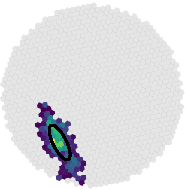
\includegraphics[height=2.8cm]{eventdisplay.pdf}};} ] (18,3.5) circle (1.5);

    \draw [draw=black!20, line width=5pt, path picture={\node at (path picture bounding box.center)
        {\includegraphics[height=4cm]{build/IceCube.jpg}};} ] (18,0) circle (1.5);

    \draw [draw=black!20, line width=5pt, path picture={\node at (path picture bounding box.center)
        {\includegraphics[height=2cm]{build/FermiLAT.jpg}};} ] (18,-3.5) circle (1.5);


    \node[
        single arrow,
        single arrow head extend=10pt,
        draw,
        inner sep=5pt,
        top color=white,
        drop shadow
        ] (B) at (10,2.5) {data taking};%

    \node[
        single arrow,
        single arrow head extend=10pt,
        draw,
        inner sep=5pt,
        top color=white,
        shape border rotate=180,
        drop shadow
        ] (C) at (10,-2.5) {measure physical quantity};%
\end{tikzpicture}
\end{document}
